\documentclass{article}

% Idioma e codificação para português brasileiro
\usepackage[brazil]{babel}
\usepackage[utf8]{inputenc}
\usepackage[T1]{fontenc}

% Margens e tamanho do papel
\usepackage[a4paper,top=2cm,bottom=2cm,left=3cm,right=3cm,marginparwidth=1.75cm]{geometry}

% Pacotes úteis
\usepackage{amsmath}
\usepackage{graphicx}
\usepackage{booktabs}
\usepackage[colorlinks=true, allcolors=blue]{hyperref}

\newcommand{\p}{\rule[-0.8mm]{20mm}{3.5mm}}

\title{Caracterização de Padrões de Depreciação Automotiva sob a Transição Energética: Uma Abordagem Baseada em Representação Espacial de Séries Temporais}
\author{Gabriel M. Brum}
\date{2026}

\begin{document}
\maketitle

\begin{abstract}
Este trabalho investiga as dinâmicas temporais de depreciação de veículos automotores a partir do conjunto de dados fipeX , com foco no impacto da inserção de veículos elétricos (EVs) no mercado brasileiro frente aos modelos convencionais a combustão interna . Metodologicamente, o estudo aborda três questões centrais: (i) a verificação de assimetrias estatísticas nas taxas de depreciação entre elétricos e a combustão de mesma faixa de valor; (ii) a análise de co-movimento e efeitos de transbordamento decorrentes de guerras de preços e marcas entrantes ; e (iii) a avaliação comparativa entre a clusterização em séries temporais 1D tradicionais e representações bidimensionais geradas via \textit{Gramian Angular Field} (GAF) e \textit{Markov Transition Field} (MTF). A proposta visa unir a caracterização econômica de novos ativos à exploração de representações espaciais como estratégia de transformação de atributos em tarefas de mineração de dados não supervisionadas.
\end{abstract}

\section{Introdução}

O mercado automotivo global e brasileiro atravessa uma transição tecnológica impulsionada pela entrada acelerada de Veículos Elétricos (EVs) \cite{alvarez2024modelagem}. Diferente dos veículos a combustão interna (ICE), cujo comportamento de depreciação histórica é consolidado e linearizado pela idade do bem, os modelos eletrificados introduzem variáveis de incerteza operacional: degradação acelerada de baterias, rápida obsolescência tecnológica, políticas tarifárias voláteis e guerras de preços \cite{gautam2024depreciation, li2026global}.

Compreender e segmentar essas trajetórias temporais não é apenas uma demanda mercadológica de precificação e análise de risco para seguradoras e instituições financeiras; constitui um problema clássico de \textit{Data Mining} voltado à mineração de séries temporais (\textit{time-series mining}) e descoberta de padrões em dados ordenados. Métodos convencionais frequentemente achatam as curvas históricas ou dependem de distâncias euclidianas 1D que falham em capturar dinâmicas não lineares, flutuações sazonais e correlações defasadas entre segmentos concorrentes \cite{schloter2022empirical}. Embora medidas de similaridade elásticas específicas para esse tipo de dado, como o \textit{Dynamic Time Warping} (DTW), ofereçam maior flexibilidade ao alinhar sequências defasadas temporalmente, elas ainda operam no domínio unidimensional e frequentemente apresentam alto custo computacional em grandes volumes de dados.

A representação convencional de séries temporais como vetores unidimensionais impõe limitações analíticas severas ao processo de mineração de dados, restringindo os algoritmos de agrupamento a métricas de distância altamente suscetíveis a variações de escala. Essa restrição metodológica fundamenta a necessidade de investigar transformações de atributos mais robustas, avaliando se representações bidimensionais geradas por \textit{Gramian Angular Fields} (GAF) ou \textit{Markov Transition Fields} (MTF) são capazes de codificar correlações cruzadas e dependências dinâmicas que escapam às métricas clássicas, como a distância Euclidiana e o DTW \cite{wu2023imaging, ulyanin2019feature}.

Sob o ponto de vista da modelagem estatística e do aprendizado de máquina, o estudo se justifica ao contrapor a eficácia de espaços latentes extraídos dessas imagens frente a métodos tradicionais de redução de dimensionalidade e seleção de atributos. A aplicação de matrizes GAF/MTF permite transpor o problema de dados tabulares temporais para o domínio de operadores de extração de padrões espaciais, abrindo caminho para testar se técnicas de aprendizado não supervisionado se beneficiam da preservação topológica dessas transformações \cite{jueco2024performance}. Com isso, o trabalho estabelece um teste empírico controlado para mensurar se a complexidade adicional dessa projeção espacial se traduz, de fato, em \textit{clusters} mais coesos e discriminantes do que os obtidos via abordagens vetoriais convencionais.

Por fim, o trabalho preenche uma lacuna relevante na análise de fenômenos de mercado ao estruturar a descoberta de padrões de desvalorização e possíveis efeitos de transbordamento decorrentes da chegada dos veículos elétricos e das montadoras chinesas \cite{li2025rise, abrardi2026market}. Ao analisar o co-movimento de preços entre matrizes energéticas concorrentes, a pesquisa vai além do agrupamento meramente exploratório e fornece um protocolo experimental rigoroso baseado em técnicas consolidadas de pré-processamento, mitigação do impacto de \textit{outliers} e validação de modelos. Dessa forma, a investigação entrega simultaneamente uma contribuição teórica sobre representação de dados ordenados na mineração de dados e uma ferramenta descritiva aplicada para precificação e gestão de risco sobre ativos automotivos.

\section{Objetivos}

\begin{itemize}
      \item \textbf{Mapear e quantificar as taxas de depreciação dos veículos elétricos:} Mensurar a velocidade e amplitude da perda de valor dos modelos eletrificados em comparação direta a veículos a combustão pareados por porte, categoria e faixa de preço de lançamento \cite{schloter2022empirical}.
      
      \item \textbf{Avaliar o efeito de transbordamento (\textit{spillover}) de marcas entrantes:} Analisar correlações temporais e possíveis quebras estruturais de preços em segmentos tradicionais após a introdução e guerra tarifária promovida por montadoras chinesas no mercado nacional \cite{li2026global, li2025rise}.

      \item \textbf{Implementar e validar o \textit{reshaping} de séries temporais em imagens 2D:} Transformar as trajetórias unidimensionais de preços de cada veículo em representações matriciais utilizando algoritmos como \textit{Gramian Angular Field} (GAF) ou \textit{Markov Transition Field} (MTF) \cite{wu2023imaging, jueco2024performance}.

      \item \textbf{Identificar e caracterizar arquétipos de desvalorização veicular:} Aplicar algoritmos de agrupamento (\textit{clustering}) sobre representações vetoriais clássicas e sobre os espaços latentes gerados a partir das imagens, identificando perfis comportamentais típicos (alta retenção, desvalorização acelerada, valorização tardia).

      \item \textbf{Comparar empiricamente a eficácia das representações:} Avaliar quantitativamente, por meio de métricas de qualidade de agrupamento (como coeficiente de Silhueta e índice Davies-Bouldin), se a transformação das séries para imagem supera as abordagens vetoriais unidimensionais tradicionais, adotando a distância Euclidiana e o \textit{Dynamic Time Warping} (DTW) como \textit{baselines} de comparação.
\end{itemize}

\section{Atividades}

\begin{itemize}
      \item \textbf{Atividade 1:} Coleta, limpeza e pré-processamento dos dados, tratamento de inconsistências/valores ausentes e estruturação temporal dos registros da base fipeX por veículo.
      
      \item \textbf{Atividade 2:} Análise exploratória e pareamento comparativo visualização das trajetórias de depreciação, cálculo de estatísticas descritivas e pareamento dos modelos elétricos com equivalentes a combustão para identificação de padrões preliminares.
      
      \item \textbf{Atividade 3:} Transformação e representação espacial (\textit{reshaping}), realizando a codificação das séries temporais 1D em representações matriciais 2D utilizando as técnicas de GAF e MTF.
      
      \item \textbf{Atividade 4:} Modelagem de agrupamento e extração de padrões aplicação e ajuste dos algoritmos de \textit{clustering} (K-Means e abordagens baseadas em densidade) sobre as representações geradas por imagem e sobre os dados vetoriais clássicos (empregando as medidas Euclidiana e DTW como \textit{baselines}).

      \item \textbf{Atividade 5:} Avaliação experimental, interpretação e escrita final com o cálculo das métricas de validação de agrupamento, análise dos arquétipos comportamentais descobertos e consolidação dos resultados no artigo final.
\end{itemize}
  
\section{Resultados}

Nesta seção serão apresentados os resultados das etapas iniciais da pesquisa, focados na higienização, transformação e redução do escopo analítico dos dados.

\subsection{Atividade 1: Pré-processamento e Limpeza de Dados}

A base de dados bruta (fipeX) foi carregada contendo originalmente mais de 9,2 milhões de registros. Como etapa inicial de limpeza estrutural, instâncias inteiramente duplicadas e registros com o atributo \texttt{valor\_centavos} igual a zero foram removidos. O escopo do projeto foi então restrito ao segmento de interesse, aplicando-se um filtro para manter apenas os registros com \texttt{tipo\_veiculo} correspondente a carros, o que reduziu a base para aproximadamente 3,3 milhões de instâncias.

Para viabilizar a análise de séries temporais, os atributos de \texttt{ano\_referencia} e \texttt{mes\_referencia} foram agregados em uma única variável \texttt{data\_referencia}. Além disso, realizou-se a seleção de atributos (\textit{feature selection}) descartando colunas redundantes, como \texttt{valor\_formatado} e \texttt{nome\_combustivel}.

Durante o pré-processamento, observou-se que uma quantidade expressiva de registros referentes a veículos novos (Zero KM) apresentava valores ausentes na coluna \texttt{ano\_modelo}, um artefato do formato textual da Tabela FIPE. Para evitar o descarte sumário desses registros e a consequente perda do preço base de lançamento — ponto de partida fundamental ($t=0$) para a construção das séries temporais de depreciação —, aplicou-se uma técnica de imputação baseada em conhecimento de domínio \cite{tan2019introduction}. O \texttt{ano\_modelo} desses veículos foi inferido e preenchido com o ano correspondente extraído da sua \texttt{data\_referencia}. Tal procedimento assegura o alinhamento de fase e a correta ancoragem da idade inicial do ativo em zero, eliminando o viés de seleção que ocorreria caso todos os preços de lançamento fossem excluídos do \textit{dataset}.

\subsection{Atividade 2: Análise Exploratória e Redução de Escopo}

Para garantir a coesão das séries temporais e evitar vieses macroeconômicos e mercadológicos, foram aplicadas heurísticas de filtragem baseadas na exploração visual e quantitativa dos dados. A Figura \ref{fig:temporal_log} ilustra a distribuição logarítmica das avaliações ao longo do tempo separadas por matriz energética, enquanto a Figura \ref{fig:idade_veiculos} apresenta a densidade populacional baseada na idade calculada de cada veículo no momento de sua cotação.

\begin{figure}[htpb]
    \centering
    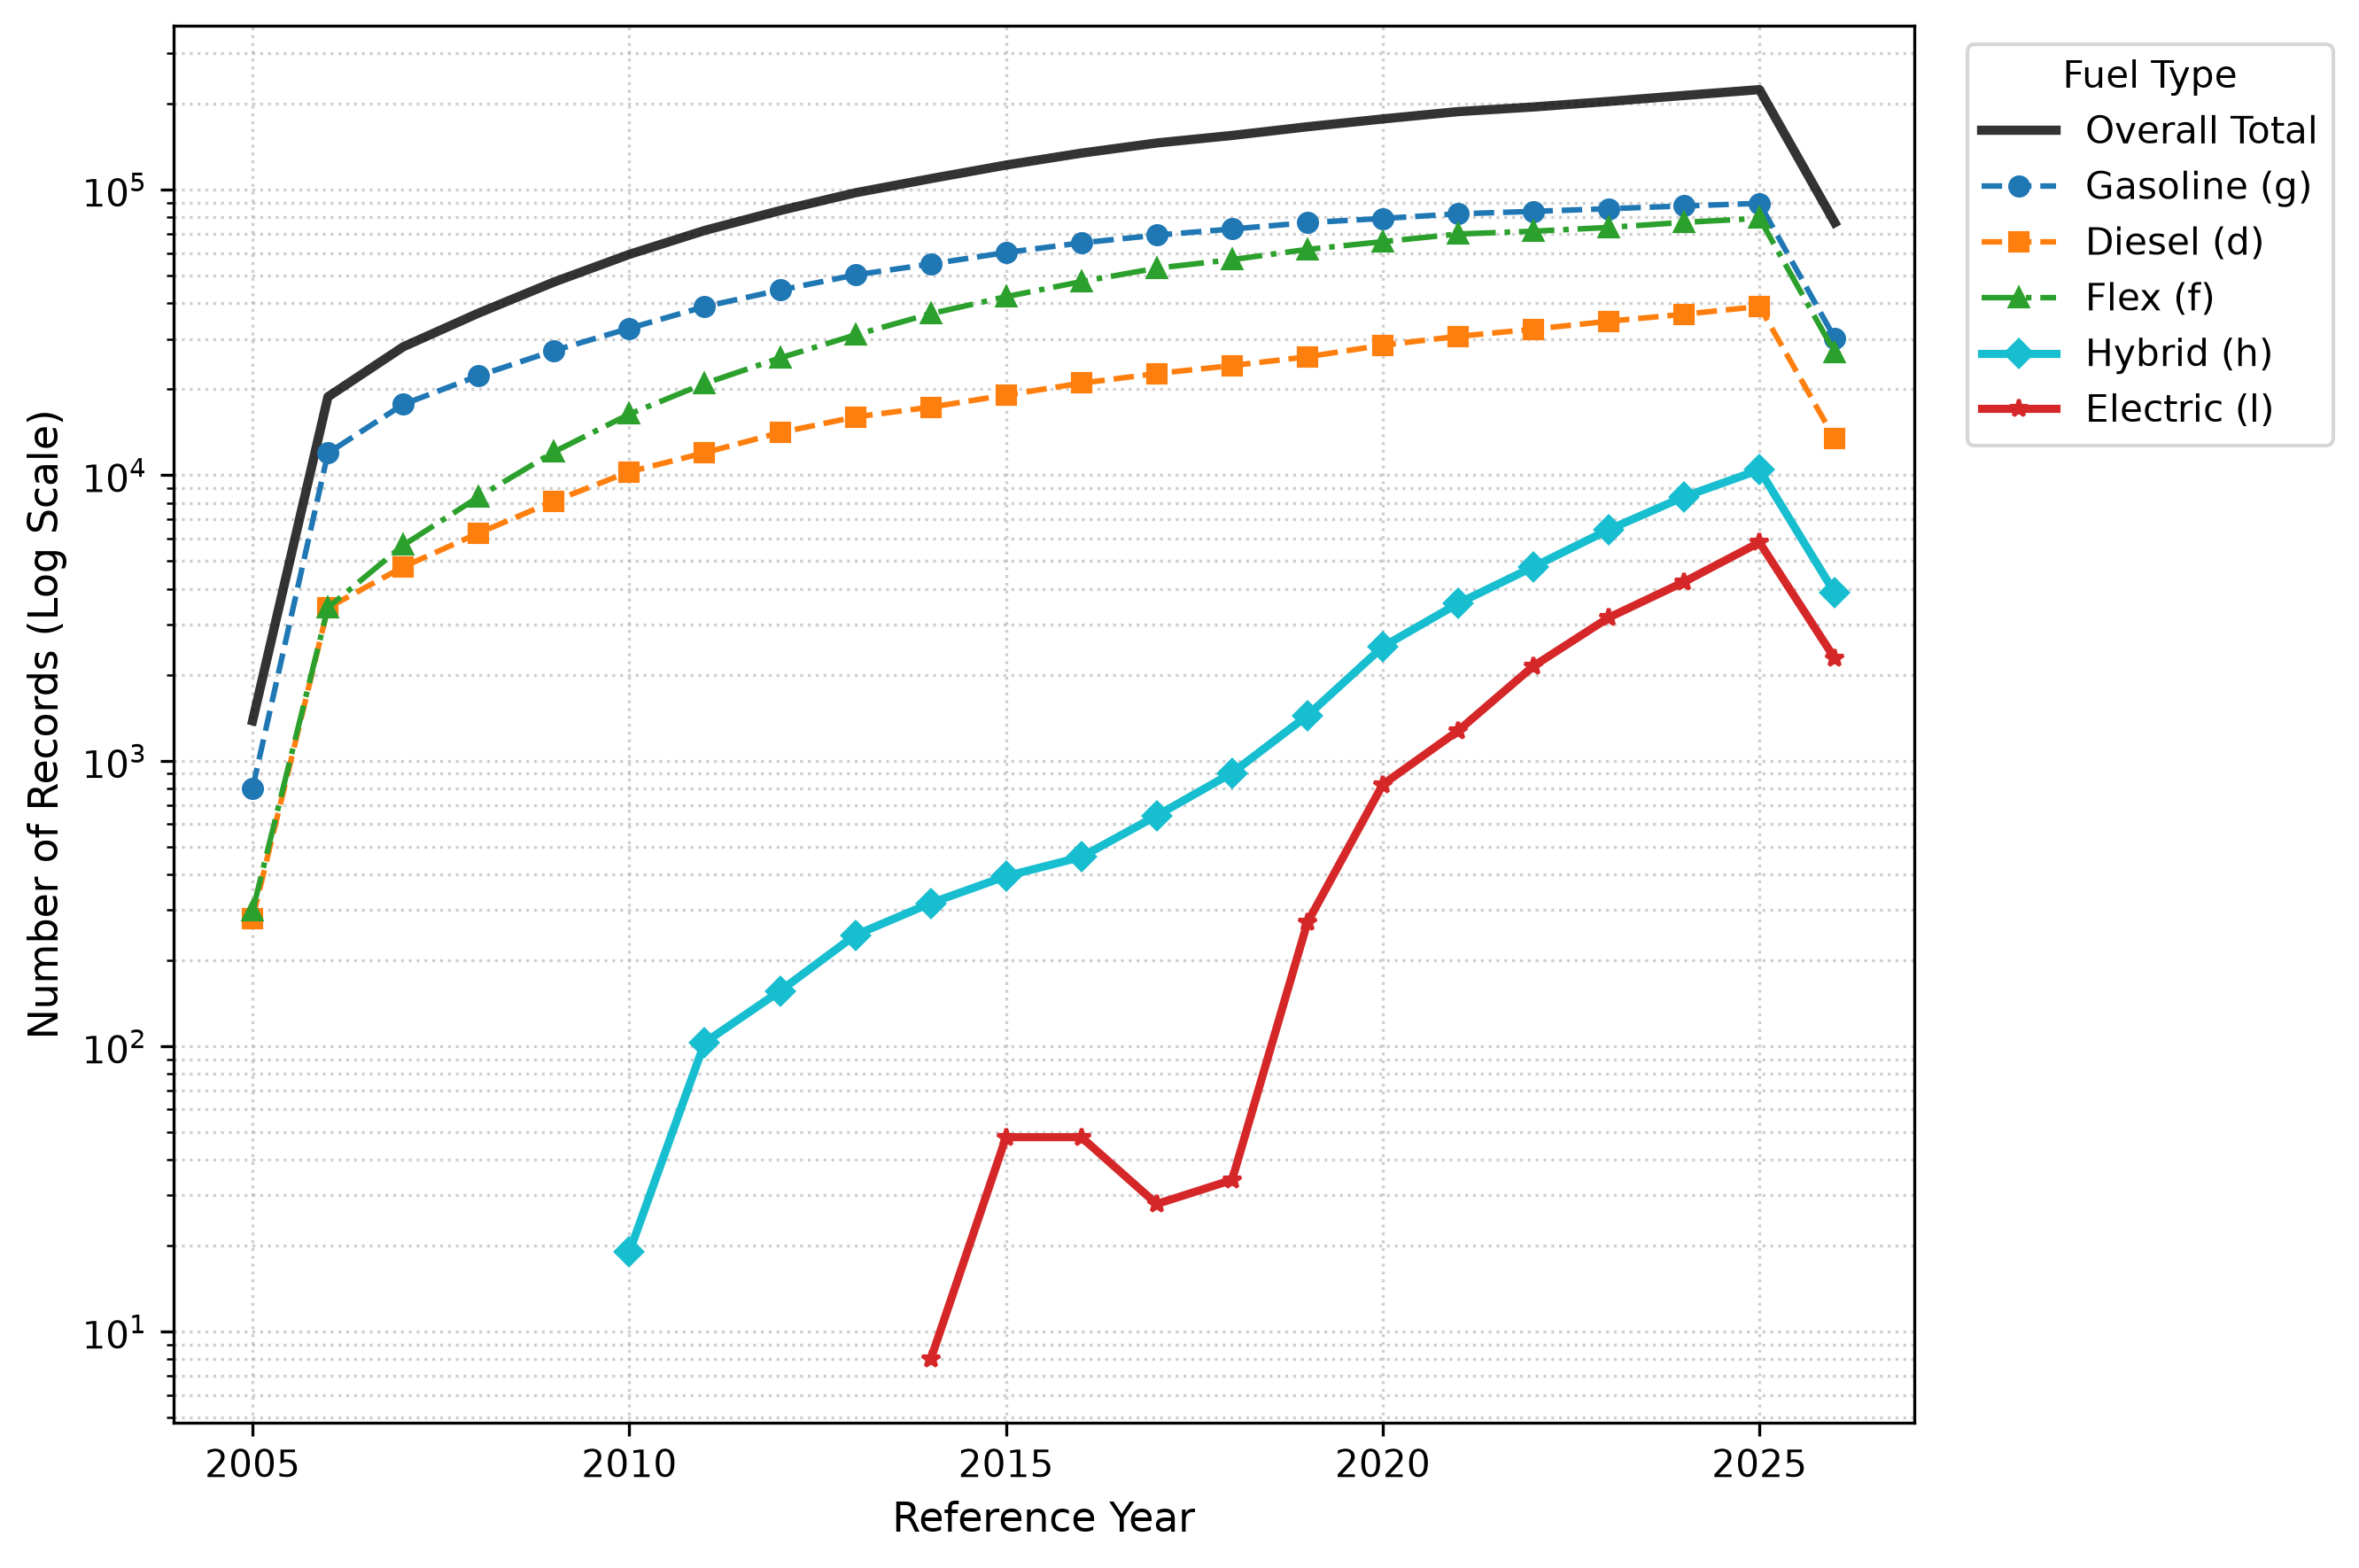
\includegraphics[width=1.0\columnwidth]{../../output/temporal_distribution_log.png}
    \caption{Distribuição temporal logarítmica da quantidade de registros por tipo de combustível (escala logarítmica).}
    \label{fig:temporal_log}
\end{figure}

Analisando a distribuição de marcas e combustíveis, identificou-se que veículos movidos a gás natural e álcool puro possuíam uma representatividade marginal e falta de variedade de montadoras. Por conta disso, decidiu-se remover essas categorias, visto que a diversidade da frota é um fator de controle crítico na análise comparativa de depreciação \cite{schloter2022empirical}. 

Para evitar o viés de acúmulo temporal (onde veículos antigos parecem ter um portfólio maior simplesmente por estarem há mais meses na base), a relevância das montadoras foi mensurada contando-se os modelos de veículos estritamente únicos (\texttt{codigo\_fipe} + \texttt{ano\_modelo} + \texttt{sigla\_combustivel}). Definiu-se o seguinte critério de corte: foram mantidas na base apenas as marcas que apresentassem um portfólio superior a 30 veículos únicos no total ou que possuíssem, no mínimo, 15 veículos únicos eletrificados (elétricos e híbridos). Esta abordagem com múltiplos limiares justifica-se pela necessidade de tratar distribuições de frequência assimétricas em tarefas de mineração de dados, garantindo que classes raras de alto interesse — neste caso, os veículos eletrificados e as montadoras entrantes — sejam adequadamente representadas \cite{tan2019introduction}. O limiar de volume atua na filtragem de ruídos, enquanto a regra de exceção preserva as montadoras recentes como \textit{outliers} legítimos, assegurando densidade sem distorcer os padrões subjacentes \cite{tan2019introduction}.

Para evitar que o modelo compare o comportamento econômico de carros a combustão da década de 1990 com elétricos de 2020, o escopo foi restringido a uma idade máxima de 20 anos. Os veículos cujo \texttt{ano\_modelo} era inferior ao corte estipulado (lançados há mais de 20 anos) foram removidos, garantindo que a análise de \textit{spillover} ocorra num cenário mercadológico e tecnológico equiparável. A partir das amostras filtradas, separando cada faixa etária dos veículos e dentre elas separando os tipos de combustíveis de cada veículo, foi obtido os resultados apresentados na Figura \ref{fig:idade_veiculos}.

\begin{figure}[htpb]
    \centering
    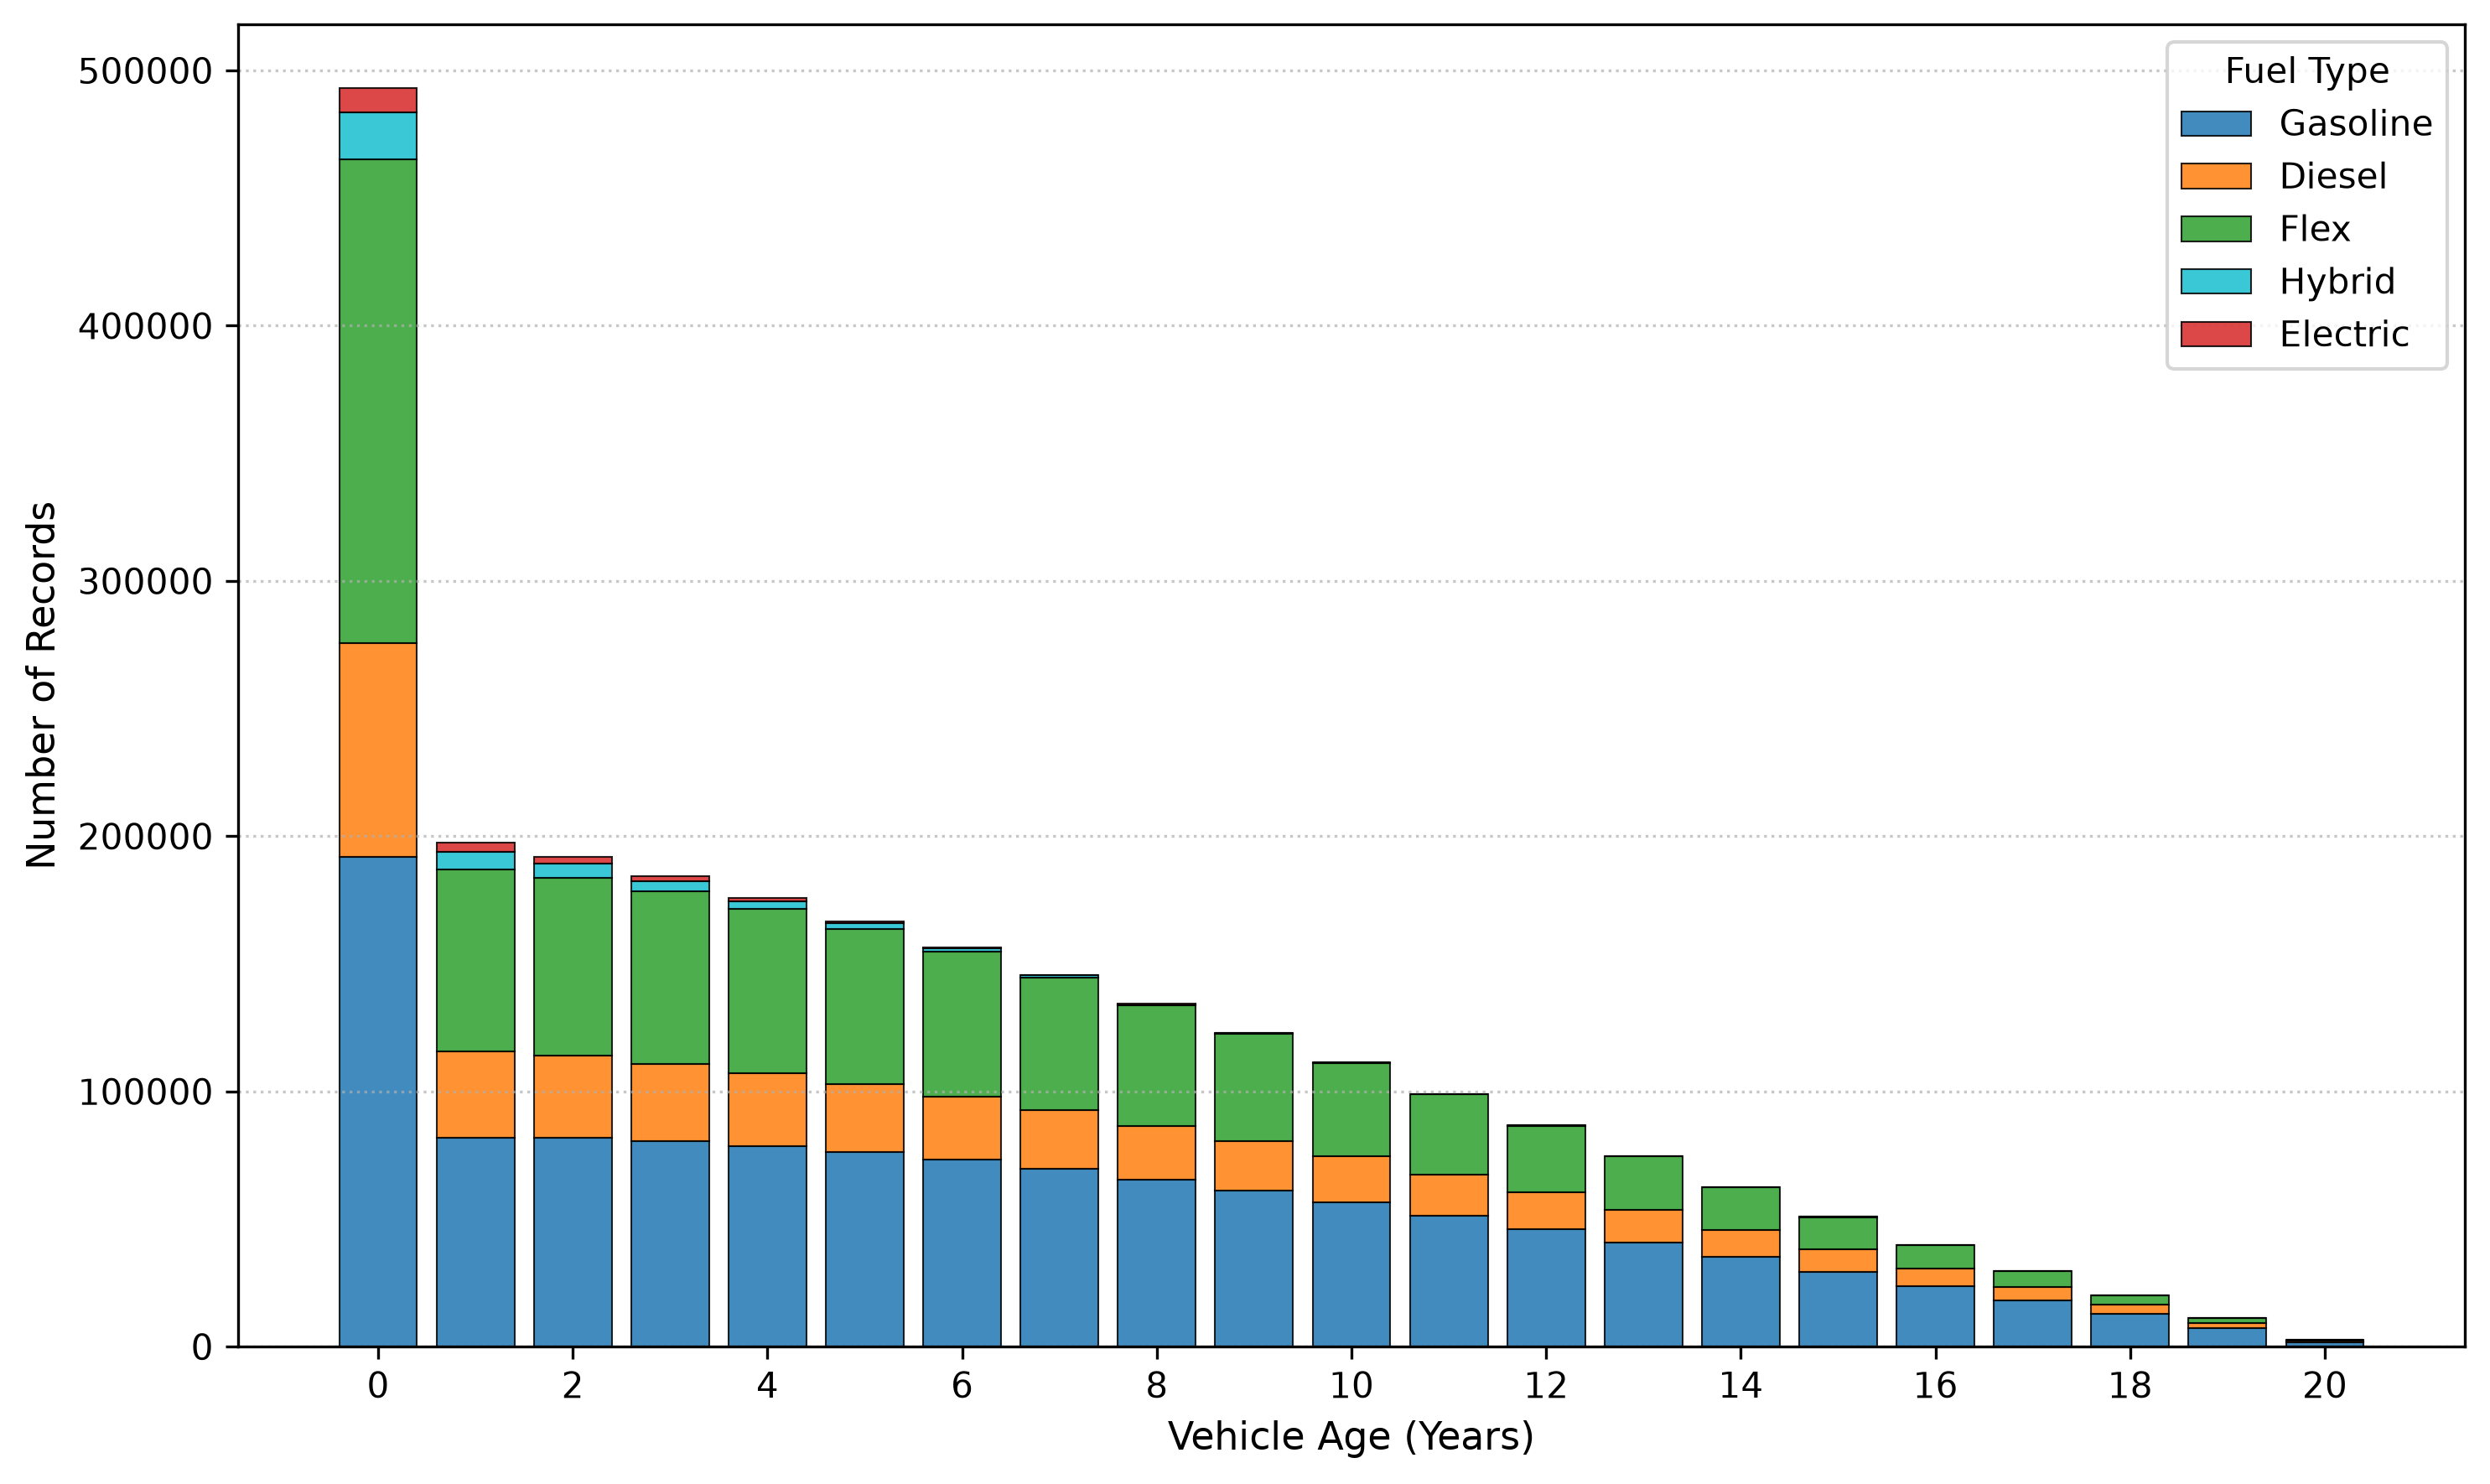
\includegraphics[width=1.0\columnwidth]{../../output/vehicle_age_distribution.png}
    \caption{Gráfico de barras empilhadas que apresenta a distribuição de registros por idade do veículo em anos, estratificada por tipo de combustível.}
    \label{fig:idade_veiculos}
\end{figure}

\subsubsection{Etapas Pendentes da Atividade 2: Retenção de Valor e Pareamento Comparativo}

Apesar da consolidação do escopo de dados e do alinhamento temporal das coortes, a conclusão da Atividade 2 exige a execução de três etapas analíticas adicionais focadas na caracterização econômica e financeira dos ativos automotivos:

\begin{itemize}
    \item \textbf{Cálculo da Retenção de Valor (Normalização):} Para viabilizar a comparação justa de desvalorização entre veículos de diferentes categorias e faixas de preço, os valores absolutos de cotação (em centavos) devem ser normalizados. Será estipulada a taxa de retenção percentual de cada veículo único, em que o preço de lançamento (quando a idade $t=0$) representará 100\% do valor de face. As idades subsequentes ($t=1, t=2, \dots$) refletirão a proporção desse valor original retido pelo mercado ao longo do tempo.

    \item \textbf{Visualização das Trajetórias Médias de Depreciação:} A partir dos dados normalizados, serão geradas e analisadas as curvas médias de depreciação agregadas por matriz energética. A projeção da idade do veículo contra a sua taxa de retenção média permitirá a identificação de assimetrias macroeconômicas preliminares, verificando de forma exploratória se os Veículos Elétricos (EVs) e Híbridos (HEVs) apresentam, de fato, um decaimento mais acentuado ou instável nos primeiros anos de uso em comparação à média dos veículos a Combustão Interna (ICE).

    \item \textbf{Pareamento Comparativo (\textit{Matching}):} Dado que o portfólio de veículos eletrificados concentra-se predominantemente nos segmentos \textit{premium} e de alta tecnologia, compará-lo diretamente à média geral da frota a combustão introduziria um forte viés de categoria. Para contornar este problema e isolar a variável da matriz energética, será aplicado um método de pareamento empírico (\textit{matching}) \cite{schloter2022empirical}. Pares de modelos equivalentes e competidores diretos no mercado brasileiro (por exemplo, \textit{hatches} ou SUVs compactos com propostas comerciais semelhantes) serão pareados e suas curvas de depreciação analisadas individualmente. Este controle metodológico garante que variações na perda de valor sejam atribuídas à motorização tecnológica e não a fatores extrínsecos de segmento.
\end{itemize}

A finalização destas análises descritivas consolidará a base empírica e a estrutura relacional das séries temporais unidimensionais, fornecendo os vetores de depreciação padronizados que serão posteriormente transformados em representações espaciais (GAF e MTF) na Atividade 3.

\bibliographystyle{plain}
\bibliography{references}

\end{document}